\documentclass{article}
\usepackage{tikz}
\usetikzlibrary{arrows.meta}

\begin{document}

\begin{figure}[h]
    \centering
    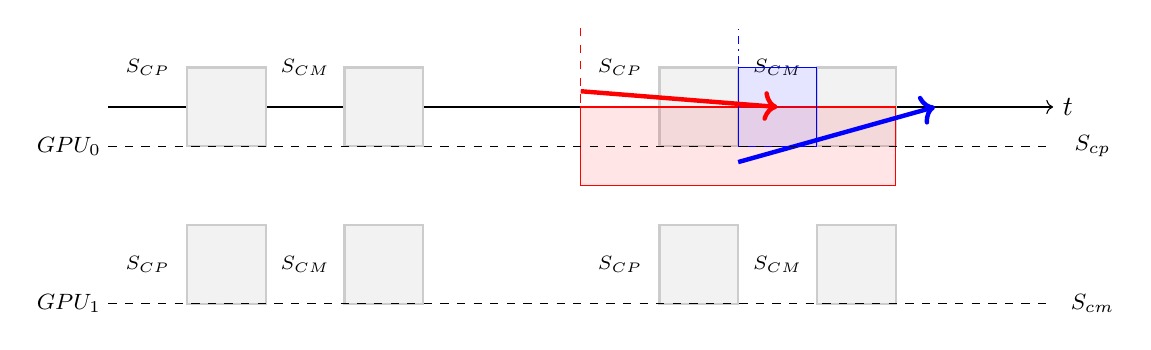
\begin{tikzpicture}
        \draw[->] (0, 0) -- (12, 0) node[right] {$t$};
        
        % GPU 0
        \foreach \i/\s in {1/CP, 3/CM, 7/CP, 9/CM} {
            \filldraw[fill=black!5, draw=black!20, thick] (\i, -0.5) rectangle ++(1, 1);
            \node at (\i-0.5, 0.5) {\scriptsize $S_{\s}$};
        }
        
        % GPU 1
        \foreach \i/\s in {1/CP, 3/CM, 7/CP, 9/CM} {
            \filldraw[fill=black!5, draw=black!20, thick] (\i, -2.5) rectangle ++(1, 1);
            \node at (\i-0.5, -2) {\scriptsize $S_{\s}$};
        }
        
        % Inter-rank synchronization (red dashed line)
        \filldraw[red, fill opacity=0.1] (6, -1) rectangle ++(4, 1);
        \draw[red, dashed] (6, -1) -- (6, 1);
        
        % Intra-rank/inter-stream synchronization (blue dotted line)
        \filldraw[blue, fill opacity=0.1] (8, -0.5) rectangle ++(1, 1);
        \draw[blue, dash dot] (8, -0.5) -- (8, 1);
        
        % Arrows indicating data dependencies
        \draw[->, ultra thick, red] (6, 0.2) -- (8.5, 0);
        \draw[->, ultra thick, blue] (8, -0.7) -- (10.5, 0);
        
        % Labels
        \node at (-0.5, -0.5) {\footnotesize $GPU_0$};
        \node at (-0.5, -2.5) {\footnotesize $GPU_1$};
        
        \node at (12.5, -0.5) {\footnotesize $S_{cp}$};
        \node at (12.5, -2.5) {\footnotesize $S_{cm}$};
        
        \draw[dashed] (0, -0.5) -- (12, -0.5);
        \draw[dashed] (0, -2.5) -- (12, -2.5);
    \end{tikzpicture}
    \caption{Two types of synchronization: inter-rank synchronization (red dashed line) and intra-rank/inter-stream synchronization (blue dotted line). For simplicity, we assume two GPUs and two streams ($S_{cp}$ and $S_{cm}$, for compute and communication respectively) per GPU, while CPU op calls are omitted in the plot. GPU kernels are represented by rectangles, and arrows indicate the data dependency between compute and communication kernels.}
    \label{fig:synchronization_diagram}
\end{figure}

\end{document}